% Style follows ../class2/resume2PT26.tex.
% Build in this directory (run twice for page references):
% pdflatex -interaction=nonstopmode -halt-on-error resume8PT26.tex
% Topics follow the syllabus in ../class1/class1PT26.tex.
% Content adapted from ../lectureNote.tex and ../lectureNotes.tex.
\documentclass[a4paper,10pt,pdflatex,ja=standard,jafont=ipaex-type1,
  magstyle=real,scale=1]{bxjsarticle}
\usepackage{lmodern}
\usepackage{amsmath,amssymb,mathtools}
\usepackage{geometry}
\geometry{reset,left=22mm,right=22mm,top=20mm,bottom=17mm,
  headheight=13pt,headsep=6mm,footskip=10mm}
\usepackage{xcolor}
\usepackage{enumitem}
\usepackage{array,booktabs,tabularx}
\usepackage{tikz}
\usepackage{fancyhdr}
\usepackage{hyperref}
\definecolor{ink}{HTML}{193A5C}
\definecolor{accent}{HTML}{237D82}
\definecolor{soft}{HTML}{EAF3F3}
\definecolor{muted}{HTML}{52616B}
\newcommand{\coursename}{確率論と統計学 I}
\hypersetup{unicode=true,colorlinks=true,urlcolor=accent,linkcolor=ink,
  pdfauthor={中島秀太},pdftitle={第8回：確率変数列の収束}}
\pagestyle{fancy}
\fancyhf{}
\fancyhead[L]{\small\color{ink}\coursename{}・授業要約と演習}
\fancyhead[R]{\small\color{ink}第8回}
\fancyfoot[C]{\small\color{ink}\thepage/\pageref*{lastpage}}
\renewcommand{\headrulewidth}{0.3pt}
\setlength{\parindent}{0pt}
\setlength{\parskip}{2pt}
\setlength{\abovedisplayskip}{4pt}
\setlength{\belowdisplayskip}{4pt}
\setlength{\abovedisplayshortskip}{3pt}
\setlength{\belowdisplayshortskip}{4pt}
\setlist[itemize]{leftmargin=1.8em,itemsep=1pt,topsep=2pt,parsep=0pt}
\setlist[enumerate]{leftmargin=2em,itemsep=3pt,topsep=3pt,parsep=0pt}
\newcommand{\topic}[1]{\par\vspace{5pt}
  {\large\sffamily\mdseries\color{accent}#1}\par\vspace{2pt}}
\newcommand{\handouttitle}[1]{%
  \begin{center}
    {\Large\color{ink}#1}\par\vspace{3mm}
    {\color{accent}\rule{0.88\linewidth}{0.7pt}}
  \end{center}\vspace{-2mm}}
\newcommand{\keybox}[1]{\par\vspace{3pt}\begingroup
  \setlength{\fboxsep}{5pt}
  \colorbox{soft}{\parbox{\dimexpr\linewidth-2\fboxsep\relax}{#1}}%
  \endgroup\par\vspace{2pt}}
\newcommand{\examplelabel}[1]{{\sffamily\mdseries\color{ink}#1}}
\newcommand{\columnheading}[1]{\par\vspace{5pt}
  {\fontsize{11pt}{15pt}\selectfont\sffamily\mdseries\color{accent}#1}\par\vspace{2pt}}
\newcommand{\columnstart}[1]{\clearpage
  \setlength{\parskip}{2.5pt}
  \fancyhead[L]{\small\color{ink}\coursename{}・発展的内容}
  {\small\sffamily\mdseries\color{accent}発展的内容}\par\vspace{4pt}
  {\Large\color{ink}#1}\par\vspace{2pt}
  {\color{accent}\rule{\linewidth}{0.7pt}}\par\vspace{4pt}}
\newcommand{\F}{\mathcal F}
\newcommand{\R}{\mathbb R}
\newcommand{\N}{\mathbb N}
\newcommand{\E}{\mathbb E}
\newcommand{\Var}{\operatorname{Var}}
\newcommand{\Cov}{\operatorname{Cov}}
\newcommand{\ind}{\mathrm{1}}
\newcommand{\iid}{\text{独立同分布}}
\begin{document}
\fontsize{10pt}{13.5pt}\selectfont
\begingroup
\fancyhead[L]{\small\color{ink}\coursename{}・前回の演習解答}
\handouttitle{第7回\quad 演習問題の解答}

\topic{演習1：幾何分布の特性関数}
$0<p<1$、$q=1-p$、$P(X=k)=pq^{k-1}$（$k\ge1$）とする。
$|qe^{it}|=q<1$ なので、絶対収束する等比級数を用いて
$$
  \varphi_X(t)=\sum_{k=1}^\infty pq^{k-1}e^{itk}
    =\frac{pe^{it}}{1-qe^{it}}\qquad(t\in\R).
$$
分母は $|1-qe^{it}|\ge1-q=p>0$ を満たし、実数 $t$ について消えない。

\topic{演習2：対称な一様分布の特性関数}
$X\sim\mathrm U(-a,a)$（$a>0$）なら、$t\ne0$ に対し
$$
  \varphi_X(t)=\frac1{2a}\int_{-a}^a e^{itx}\,dx
    =\frac{e^{iat}-e^{-iat}}{2ait}=\frac{\sin(at)}{at}.
$$
$t=0$ では定義から $\varphi_X(0)=1$。
$\sin u/u\to1$（$u\to0$）より、この値で原点でも連続になる。

\topic{演習3：独立な正規確率変数の和}
独立な $X\sim N(m_1,v_1)$、$Y\sim N(m_2,v_2)$（$v_1,v_2>0$）について
$$
  \begin{aligned}
    \varphi_{X+Y}(t)&=\varphi_X(t)\varphi_Y(t)\\
      &=e^{im_1t-v_1t^2/2}e^{im_2t-v_2t^2/2}
       =e^{i(m_1+m_2)t-(v_1+v_2)t^2/2}.
  \end{aligned}
$$
これは $N(m_1+m_2,v_1+v_2)$ の特性関数であり、一意性から
$X+Y\sim N(m_1+m_2,v_1+v_2)$ と分かる。

\topic{演習4：Gauss 核による平滑化の一様収束}
$f\in C_c(\R)$、$q_\varepsilon(y)=e^{-y^2/(2\varepsilon^2)}/(\sqrt{2\pi}\varepsilon)$ とする。
$\int q_\varepsilon=1$ なので、$\delta>0$ に対し
$$
  \begin{aligned}
    |(f*q_\varepsilon)(x)-f(x)|
      &\le\int_\R|f(x-y)-f(x)|q_\varepsilon(y)\,dy\\
      &\le\sup_{|u-v|\le\delta}|f(u)-f(v)|
        +2\|f\|_\infty\int_{|y|>\delta}q_\varepsilon(y)\,dy.
  \end{aligned}
$$
右辺は $x$ によらず、上限をとれば設問の評価となる。
$f$ の一様連続性から第1項は $\delta\downarrow0$ で消える。
固定した $\delta$ に対し、第2項の積分は $N(0,\varepsilon^2)$ の尾確率で、
Chebyshev の不等式により $\varepsilon^2/\delta^2$ 以下となる。
先に $\delta$ を小さく選び、次に $\varepsilon\downarrow0$ とすれば一様収束を得る。
\clearpage
\endgroup

\handouttitle{第8回\quad 確率変数列の収束}
\keybox{概収束は各標本での長期的な振る舞い、確率収束は各時点での誤差確率を見る。
量化の順序を区別し、どちらの条件が必要かを考えよう。}

\topic{概収束：標本ごとに極限をとる}
以下、$X_n,X$ は同じ確率空間 $(\Omega,\F,P)$ 上の実数値確率変数とする。
$X_n$ が $X$ に概収束するとは
$$P(\{\omega:X_n(\omega)\to X(\omega)\})=1$$
となることであり、$X_n\to X$ a.s. と書く。
確率 $0$ の例外を除き、一つの $\omega$ を固定した数列が収束する。
$\varepsilon>0$ に対して
$$A_n(\varepsilon)=\{|X_n-X|>\varepsilon\}$$
とおくと、概収束は
$$P\left(\bigcap_{N=1}^\infty\bigcup_{n\ge N}A_n(1/m)\right)=0
 \qquad(m=1,2,\ldots)$$
と同値である。「誤差が一定以上になること」が無限回は起こらない、という条件である。

\topic{確率収束：大きな誤差の確率が消える}
$X_n$ が $X$ に確率収束するとは
$$P(|X_n-X|>\varepsilon)\longrightarrow0
 \qquad(\forall\varepsilon>0)$$
となることであり、$X_n\xrightarrow{P}X$ と書く。
各時点 $n$ で誤差の大きい標本の割合は小さくなるが、
その例外となる標本が $n$ ごとに入れ替わることは許される。

\topic{概収束なら確率収束}
$X_n\to X$ a.s. なら、固定した $\varepsilon>0$ について
$$\ind_{\{|X_n-X|>\varepsilon\}}\to0\ \text{a.s.},\qquad
 0\le\ind_{\{|X_n-X|>\varepsilon\}}\le1.$$
優収束定理より
$$P(|X_n-X|>\varepsilon)=\E[\ind_{\{|X_n-X|>\varepsilon\}}]\to0.$$
逆向きは一般には成立しない。次ページの例では、誤差確率は小さくなるが、
各標本では大きな誤差が無限回生じる。

\topic{極限の一意性}
$X_n\xrightarrow{P}X$ かつ $X_n\xrightarrow{P}Y$ なら、任意の $\varepsilon>0$ に対し
$$P(|X-Y|>\varepsilon)
 \le P(|X-X_n|>\varepsilon/2)+P(|X_n-Y|>\varepsilon/2)\to0.$$
$\varepsilon=1/m$ を可算個とれば $P(X=Y)=1$ となる。
確率変数の極限は、零集合上での違いを除いて一意である。

\newpage
\topic{確率収束しても概収束しない：動く区間}
$\Omega=[0,1)$ に一様確率を入れる。
$n=2^m+k$（$m\ge0$、$0\le k<2^m$）と一意に書き、
$$X_{2^m+k}(\omega):=\ind_{[k2^{-m},(k+1)2^{-m})}(\omega)$$
と定める。区間を左から右へ走査し、一巡ごとに長さを半分にする。
各 $0<\varepsilon<1$ に対し
$$P(|X_{2^m+k}|>\varepsilon)=2^{-m}\longrightarrow0.$$
したがって $X_n\xrightarrow{P}0$。
一方、各 $\omega$ はどの段 $m$ でもちょうど一つの区間に入るため、
値 $1$ が無限回現れる。値 $0$ も無限回現れ、どの $\omega$ でも収束しない。

\topic{和と積の確率収束}
$X_n\xrightarrow{P}X$、$Y_n\xrightarrow{P}Y$ なら
$$X_n+Y_n\xrightarrow{P}X+Y,\qquad X_nY_n\xrightarrow{P}XY.$$
和には三角不等式と和集合の確率評価を使う。
積については、$|X|,|Y|\le M$ かつ
$|X_n-X|,|Y_n-Y|\le\delta$ という事象上で
$$|X_nY_n-XY|
 \le|X_n-X|\,|Y_n|+|X|\,|Y_n-Y|
 \le\delta(2M+\delta).$$
まず $M$ を大きくして $P(|X|>M)+P(|Y|>M)$ を小さくし、
次に $\delta$ を小さく選び、最後に $n\to\infty$ とする。
概収束の場合は、共通の確率 $1$ の集合上で通常の数列の演算を使えばよい。

\topic{確率収束から概収束する部分列を取り出す}
$X_n\xrightarrow{P}X$ なら、$n_k$ を増加するように選んで
$$P(|X_{n_k}-X|>2^{-k})\le2^{-k}$$
とできる。右辺の和が有限なので、Borel--Cantelli の補題により
$|X_{n_k}-X|>2^{-k}$ は a.s. 有限回しか起こらない。
よって $X_{n_k}\to X$ a.s.。列全体の概収束とは区別する必要がある。

\topic{期待値の収束は別に確認する}
$p>0$ に対し $\E|X_n-X|^p\to0$ なら、Markov の不等式から確率収束する。
その逆は一般に成り立たない。$X_n=n\ind_{(0,1/n)}$ を $\Omega=(0,1)$ 上で考えると
$X_n\to0$ a.s. だが $\E|X_n|=1$。
確率収束や概収束だけで、非有界な関数の期待値を極限と交換してはいけない。

\begin{center}
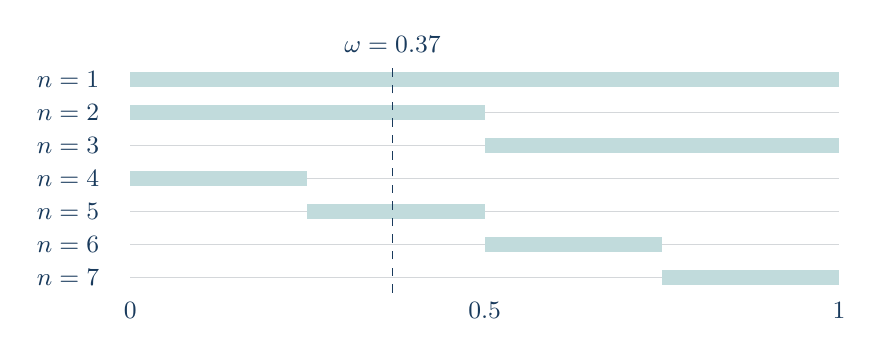
\begin{tikzpicture}[x=9cm,y=0.42cm,font=\small]
 \foreach \n/\a/\b/\y in {1/0/1/6,2/0/0.5/5,3/0.5/1/4,
 4/0/0.25/3,5/0.25/0.5/2,6/0.5/0.75/1,7/0.75/1/0}{
   \draw[muted!25] (0,\y)--(1,\y);
   \fill[accent!28] (\a,{\y-0.22}) rectangle (\b,{\y+0.22});
   \node[left,ink] at (-0.03,\y) {$n=\n$};
 }
 \draw[ink,dashed] (0.37,-0.45)--(0.37,6.5)
   node[above] {$\omega=0.37$};
 \foreach \x in {0,0.5,1}{\node[below,ink] at (\x,-0.45) {$\x$};}
\end{tikzpicture}
\end{center}
{\small\color{muted}帯が $X_n=1$ となる区間を表す。同じ $\omega$ に沿って見ると、
区間が細くなっても値 $1$ が繰り返し現れる。}\par

\newpage
\topic{演習問題}
\begin{enumerate}[label=\arabic*.]
\item $U\sim\mathrm U(0,1)$ とし、$X_n=U^n$、$Y_n=nU^n$ とおく。
それぞれの概収束と確率収束を調べ、期待値の極限も計算せよ。
\item $X_n\xrightarrow{P}X$、$Y_n\xrightarrow{P}Y$ とする。
$aX_n+bY_n\xrightarrow{P}aX+bY$（$a,b\in\R$）を示せ。
\item 動く区間の例で $n_k=2^k$ と選ぶと、$X_{n_k}$ はどこで何に収束するか。
列全体とこの部分列の振る舞いの違いを説明せよ。
\item $P(|X_n-X|>\varepsilon)\le C_\varepsilon n^{-2}$（各 $\varepsilon>0$）なら
$X_n\to X$ a.s. を示せ。$n^{-1}$ の上界だけでも同じ証明が使えるか。
\end{enumerate}

\topic{レポート問題}
\begin{enumerate}[label=\arabic*.]
\item $X_n\xrightarrow{P}X$、$Y_n\xrightarrow{P}Y$ から
$X_nY_n\xrightarrow{P}XY$ を証明せよ。
$X,Y$ が有界であると仮定せず、尾の確率を先に抑えること。
\item 独立な $\{0,1\}$ 値確率変数 $B_n$ が $P(B_n=1)=1/(n+1)$ を満たすとする。
$B_n\xrightarrow{P}0$ を示せ。
独立な事象に対する Borel--Cantelli の補題を用い、$B_n$ が概収束しないことを示せ。
\end{enumerate}

\topic{考えるための手がかり}
確率収束では固定した時点の確率を見る。概収束では、
同じ標本に沿って無限回の時点を見渡す。
$\limsup_n A_n=\bigcap_N\bigcup_{n\ge N}A_n$ は、$A_n$ が無限回起こる事象である。
\vfill
{\small\color{muted}解答メモ：「すべての $\varepsilon$」を概収束の議論へ移す際は $\varepsilon=1/m$ を使う。}

\columnstart{小さい確率の出来事も、繰り返せば起こる}
一回ごとの失敗確率が小さくなるとき、失敗はいずれ完全になくなるだろうか。
確率収束と概収束の違いには、まれな出来事が時間の中でどう積み重なるかが現れる。

\columnheading{和が有限なら、無限回は起こらない}
事象列 $(A_n)$ に対し、和集合の確率評価から
$$P\left(\bigcup_{n\ge N}A_n\right)\le\sum_{n\ge N}P(A_n).$$
$\sum_nP(A_n)<\infty$ なら、$N\to\infty$ で右辺は $0$ になる。
したがって
$$P(A_n\text{ が無限回起こる})=0.$$
これが Borel--Cantelli の第1補題である。事象どうしの独立性は必要ない。
誤差確率の和を有限にできれば、標本ごとの収束へ進める。

\columnheading{和が無限大の場合には独立性が効く}
事象が相互独立なら、固定した $N$ に対して
$$P\left(\bigcap_{n=N}^M A_n^c\right)
 =\prod_{n=N}^M(1-P(A_n))
 \le\exp\left(-\sum_{n=N}^M P(A_n)\right).$$
$\sum_nP(A_n)=\infty$ なら $M\to\infty$ で右辺は $0$。
どの $N$ 以降にも何かが起こるので、$A_n$ は a.s. 無限回起こる。
これが独立な事象に対する第2補題である。
和が発散するだけでは、独立性なしにこの結論は出ない。

\columnheading{収束の反例を一つ作る}
独立な $B_n\in\{0,1\}$ に $P(B_n=1)=1/(n+1)$ を与える。
各時点では $P(B_n=1)\to0$ なので $B_n\xrightarrow{P}0$。
しかし確率の和は発散するため、値 $1$ は a.s. 無限回現れる。
補事象の確率の和も発散し、独立性も保たれるので値 $0$ も a.s. 無限回現れる。
よって $B_n$ は概収束しない。
「時点ごとにはまれ」と「一つの軌跡で有限回しか起こらない」は異なる条件なのである。

\columnheading{速い部分列なら標本ごとにも収束する}
同じ例で $n_k=2^k$ とすれば
$$\sum_{k\ge1}P(B_{2^k}=1)=\sum_{k\ge1}\frac1{2^k+1}<\infty.$$
第1補題から $B_{2^k}\to0$ a.s. となる。
確率収束する列から概収束する部分列を選べるという本文の定理は、
この「誤差確率の和が有限になるまで時点を間引く」考え方を一般化したものである。
どの収束を使っているかを明記すると、部分列の議論も見通しがよくなる。

\label{lastpage}
\end{document}
